%!TeX program = xelatex
\documentclass[11pt,a4paper,oneside]{ctexart}

\usepackage[left=1.95cm,right=1.95cm,top=2.05cm,bottom=2.05cm]{geometry}
\usepackage{TJUReport}
\usepackage{graphicx,booktabs,tabularx,array,multirow}
\usepackage{amsmath,amssymb,bm}
\usepackage[svgnames]{xcolor}
\usepackage{tikz}
\usetikzlibrary{arrows.meta,positioning,calc,fit,shapes.geometric}
\usepackage{caption,subcaption}
\usepackage{float}
\usepackage{needspace}
\usepackage{enumitem}
\usepackage{microtype}
\usepackage{hyperref}
\usepackage{xurl}

\definecolor{samblue}{HTML}{2B6CB0}
\definecolor{auditgold}{HTML}{D69E2E}
\definecolor{recovergreen}{HTML}{2F855A}
\definecolor{riskred}{HTML}{C53030}
\definecolor{softgray}{HTML}{F4F5F7}
\hypersetup{colorlinks=true,linkcolor=black,citecolor=black,urlcolor=samblue}
\captionsetup{font=small,labelfont=bf,skip=4pt}
\setlength{\headheight}{27pt}
\setlength{\emergencystretch}{2em}
\setlength{\parindent}{2em}
\setlength{\parskip}{0pt}
\linespread{1.16}
\setlist{nosep,leftmargin=2em}
\ctexset{
  section={format=\Large\bfseries,beforeskip=0.8ex,afterskip=0.45ex},
  subsection={format=\large\bfseries,beforeskip=0.65ex,afterskip=0.3ex},
  subsubsection={format=\normalsize\bfseries,beforeskip=0.45ex,afterskip=0.2ex}
}
\newcommand{\method}{ReAnchor-MOSE}
\newcommand{\jf}{\ensuremath{\mathcal{J}\!\&\!\mathcal{F}'}}
\newcommand{\code}[1]{\texttt{#1}}
\newcommand{\good}{\textcolor{recovergreen}{\textbf{有效}}}
\newcommand{\neutral}{\textcolor{auditgold}{\textbf{有意义但未显著增益}}}
\newcommand{\bad}{\textcolor{riskred}{\textbf{不采用}}}

\begin{document}

% ---------- cover ----------
\begin{titlepage}
  \thispagestyle{empty}
  \centering
  \vspace*{0.8cm}
  
\includegraphics[width=0.43\textwidth]{figures/tongji.png}
  \vspace{0.2cm}

  {\heiti\fontsize{24pt}{34pt}\selectfont
  面向复杂遮挡与同类干扰的\par
  训练自由视频目标分割\par}
  \vspace{0.45cm}
  {\heiti\fontsize{16pt}{24pt}\selectfont
  SAM2在MOSEv2上的复现、重锚定与多模态辅助\par}

  \vspace{1.35cm}
  \renewcommand{\arraystretch}{1.7}
  {\kaishu\large
  \begin{tabular}{r l}
    学院：& \underline{\makebox[8.0cm][c]{国豪书院}}\\
    专业：& \underline{\makebox[8.0cm][c]{数据科学与大数据技术}}\\
    学号：& \underline{\makebox[8.0cm][c]{2352190}}\\
    姓名：& \underline{\makebox[8.0cm][c]{於之翔}}\\
    课程：& \underline{\makebox[8.0cm][c]{计算机视觉}}\\
    日期：& \underline{\makebox[8.0cm][c]{2026年6月}}\\
  \end{tabular}}
  \vfill
\end{titlepage}

% ---------- abstract ----------
\begin{abstract}
MOSEv2 将视频目标分割的难点从“沿时间传播显著外观”推进到“在复杂场景中持续确认同一物理实例”：目标可能在首帧就被遮挡或仅占图像的极小区域，随后长期消失、尺度剧变，并在多个高度相似的同类对象旁重现。本文在仅使用首帧真值掩码、不训练或微调、不得访问后续真值的约束下，以 SAM~2 为稳定传播基座，设计训练自由系统 \method{}。核心思路不是继续调高或调低置信阈值，而是把推理拆分为稳定传播、不确定性审计、候选再获取、身份验证、延迟提交、有界回传和保守融合七个环节：正常区间完全保留基线；发生遮挡或身份歧义后，系统从多模型、自动掩码和局部搜索中生成高召回候选，用首帧与消失前锚点构成正例记忆、用同类对象与被拒轨迹构成困难负例记忆；候选经对象描述器、运动可达性和多帧一致性确认后，才通过 SAM~2 原生提示接口写回局部记忆。

在完整测试集上，本文的整体结构优化取得了 50.1 的 \jf{}，较 SAM2 复现基线提高约 4 个点。完成这一阶段后，剩余错误主要集中在 15 个具有代表性的困难视频。本文进一步引入 MLLM 分层调用框架，把这些样本作为提示设计与视频内容理解的上限研究：短视觉请求负责逐帧观察，深度模型负责聚合“离场—重现”“拿起—移动—放下”“向镜头运动”等事件链；语言模型只能提出搜索约束、支持或否决候选，不能直接产生掩码或单独提升锚点。对象级反馈表明，只有当语义理解被落实为正确的后续帧候选并重新驱动分割传播时，才会产生真实增益。结果说明，复杂视频分割的关键不是让模型更自信，而是给它建立传播之外的新证据通路，并严格控制新证据何时进入长期记忆。

\vspace{0.25em}
\noindent\textbf{关键词：} 视频目标分割；MOSEv2；SAM2；训练自由；重锚定；困难负例记忆；多模态大模型
\end{abstract}

\section{问题背景与研究动机}

\subsection{从掩码传播到物理实例确认}
半监督视频目标分割（Video Object Segmentation, VOS）给定首帧实例掩码，要求预测同一实例在后续帧中的像素区域。DAVIS 建立了以区域与边界质量为核心的传统评测范式，YouTube-VOS 则把训练和评测扩展到更大规模视频\cite{perazzi2016davis,xu2018youtubevos}。时空记忆网络 STM 首次把历史帧及其掩码写入外部记忆，并以当前帧为 query 做稠密匹配\cite{oh2019stm}；XMem 进一步用感知、工作和长期记忆控制长视频中的容量与遗忘\cite{cheng2022xmem}；Cutie 又以对象查询进行自上而下的对象级读取，缓解纯像素匹配受干扰物影响的问题\cite{cheng2024cutie}。这条发展脉络说明，VOS 的关键始终不仅是单帧分割，还包括如何组织跨帧证据。

MOSE/MOSEv2 集中加入长遮挡、消失重现、极小目标、多镜头、阴影反射和密集同类干扰\cite{ding2023mose,ding2025mosev2}。此时，“当前候选像目标”与“当前候选就是首帧指定实例”不再等价。它也是本文选择复现 SAM2 并继续改造其记忆结构，而不是只做边界后处理的直接原因。

Segment Anything 以可提示分割和大规模数据引擎建立了通用分割基础模型范式\cite{kirillov2023sam}。SAM~2 在此基础上加入流式视频记忆：当前帧视觉特征通过 memory attention 读取历史 mask memory 与 object pointer，mask decoder 输出结果，再由 memory encoder 写回历史\cite{ravi2024sam2}。这一结构高效且可交互，却有明显的自回归风险：一旦模型在某帧误跟到同类干扰物，错误掩码会被当成未来证据，形成“稳定但错误”的轨迹。SAM2Long 的多路径记忆树\cite{ding2024sam2long}与 DAM4SAM 的干扰感知记忆\cite{videnovic2024dam4sam}都说明，复杂视频的核心瓶颈已从单帧边界精度转向长期记忆治理和身份恢复。

\subsection{任务形式化与评价指标}
给定视频 $\mathcal V=\{I_t\}_{t=0}^{T-1}$ 和首帧 $K$ 个实例标签 $Y_0$，在固定模型参数 $\theta$、不访问 $Y_{t>0}$ 的条件下预测
\begin{equation}
  \hat Y_{1:T-1}=f(\mathcal V,Y_0;\theta),\qquad \theta\ \text{不更新}.
\end{equation}
区域指标 $\mathcal J$ 为交并比，边界指标 $\mathcal F'$ 衡量轮廓匹配，官方 \jf{} 综合两者。本文还额外要求\textbf{身份一致性}：输出非空掩码必须对应首帧同一物理对象，而不是任意同类对象。

\subsection{观察、洞见与贡献}
逐帧审查表明，困难样本主要落入五类：长遮挡后的重现、密集同类实例、首帧残缺或位于边缘、面积不足图像 $1\%$ 的极小目标，以及快速运动/转体带来的外观突变。由此得到本文最重要的洞见：
\begin{quote}
\small\textbf{掩码质量、类别相似和实例身份是三个层次的命题。}可靠性门控只能判断“这个掩码是否稳定”，不能证明“它是不是原来的那个对象”；要恢复身份，必须在传播路径之外重新获得候选，并让候选在写入记忆前接受正负身份与时空一致性的联合验证。
\end{quote}
本文贡献可概括为三点：第一，把 SAM2 的单路径自回归改造成“传播—审计—再获取—验证—提交—回滚”闭环；第二，以对象为中心同时维护正锚点和同类困难负例，并用延迟提交避免单帧误判污染长期记忆；第三，把 MLLM 限定为事件解释和候选支持/否决模块，以结构化多帧推理辅助 15 个难例，同时保留像素模型的最终决定权。

\section{训练自由架构优化}

\subsection{整体设计：稳定路径之外建立恢复路径}
结构设计来自三步递进的判断。首先，STM、XMem 和 SAM2 证明记忆传播是 VOS 的有效主干，因此不应在目标连续可见时轻易替换它；其次，Cutie、SAM2Long 与 DAM4SAM 表明像素匹配、单路径选择和只保存正例都会在同类干扰下失效，因此恢复阶段必须引入对象级表示、多分支假设和困难负例；最后，SAM2 原生支持后续提示，意味着经过验证的后续帧锚点可以真正改变未来推理，而不是停留在输出后处理。由此，本文没有堆叠一个统一评分器，而是把“提出候选、确认身份、改写记忆”拆成权限不同的环节。

图~\ref{fig:architecture} 给出系统结构。蓝色为原始 SAM2 稳定路径；黄色模块只在不确定事件出现时工作；绿色模块完成身份恢复；红色模块控制提交风险。与“每帧都套一层复杂控制器”不同，本文只在必要处增加计算，因此既减少对稳定视频的扰动，也使每次改动都可审计。

\begin{figure}[H]
\centering
\resizebox{0.98\textwidth}{!}{
\begin{tikzpicture}[
 node distance=5mm and 6mm,
 block/.style={rounded corners,draw,thick,minimum height=10mm,align=center,text width=21mm,fill=white},
 arrow/.style={-{Stealth[length=2mm]},thick},
 note/.style={rounded corners,draw,dashed,align=center,text width=28mm,fill=softgray,font=\scriptsize}
]
\node[block,draw=samblue,fill=samblue!8] (input) {首帧 GT\\视频帧};
\node[block,draw=samblue,fill=samblue!8,right=of input] (sam) {SAM2\\稳定传播};
\node[block,draw=auditgold,fill=auditgold!10,right=of sam] (audit) {三态审计\\稳定/歧义/恢复};
\node[block,draw=auditgold,fill=auditgold!10,right=of audit] (cand) {高召回\\候选池};
\node[block,draw=recovergreen,fill=recovergreen!10,right=of cand] (verify) {正负记忆\\身份验证};
\node[block,draw=recovergreen,fill=recovergreen!10,right=of verify] (commit) {延迟提交\\伪锚点};
\node[block,draw=samblue,fill=samblue!8,right=of commit] (reprop) {SAM2\\有界重传播};
\node[block,draw=riskred,fill=riskred!8,right=of reprop] (fusion) {逐对象融合\\差异回滚};
\node[note,below=8mm of cand] (ledger) {对象时序账本：可见性、运动、遮挡、同类干扰物};
\node[note,below=8mm of verify] (mllm) {后续难例扩展：MLLM 逐帧观察 $\rightarrow$ 事件链聚合};
\draw[arrow] (input)--(sam); \draw[arrow] (sam)--(audit); \draw[arrow] (audit)--(cand);
\draw[arrow] (cand)--(verify); \draw[arrow] (verify)--(commit); \draw[arrow] (commit)--(reprop); \draw[arrow] (reprop)--(fusion);
\draw[arrow,dashed] (audit)--(ledger); \draw[arrow,dashed] (ledger)--(verify); \draw[arrow,dashed] (mllm)--(verify);
\draw[arrow,dashed,bend left=22] (audit) to node[above,font=\scriptsize]{稳定区间直通} (fusion);
\end{tikzpicture}}
\caption{ReAnchor-MOSE 总体架构。系统不是替换 SAM2，而是在其单路径传播失效时建立可回滚的身份恢复支路。}
\label{fig:architecture}
\end{figure}

\subsection{三态审计与锚点库}
对每个对象独立维护 $s_t\in\{\texttt{stable},\texttt{ambiguous},\texttt{recovery}\}$。审计量包括连续空帧数、objectness、预测 IoU、面积突变、中心运动残差、不同来源分歧和身份 margin。稳定状态完全沿用 SAM2；出现遮挡、来源冲突或运动不可达时进入 ambiguous，此时允许候选进入 provisional branch，但禁止写长期记忆；确认主路径失效后进入 recovery，触发全局/局部再获取。

每个对象的记忆库写为
\begin{equation}
\mathcal B_k=\{A_k^0,\mathcal P_k,\mathcal R_k,\mathcal N_k\},
\end{equation}
其中 $A_k^0$ 为首帧锚点，$\mathcal P_k$ 为消失前高质量正例，$\mathcal R_k$ 为已验证重现锚点，$\mathcal N_k$ 为困难负例。负例不是普通背景，而是同帧其他对象、被时序周期检查拒绝的轨迹、附近同类候选、context ring 和已知错误来源。候选 $c$ 的身份判据使用正负差值
\begin{equation}
m(c)=\max_{p\in\mathcal P_k\cup\mathcal R_k}\cos(f_c,f_p)-\max_{n\in\mathcal N_k}\cos(f_c,f_n),
\label{eq:margin}
\end{equation}
而非只看“像不像正例”。$f$ 由 DINOv2 patch token\cite{oquab2024dinov2}、SAM2 Hiera 特征和颜色/形状统计组合。极小目标在特征网格内不足三个 token 时，改用扩大局部框的 crop descriptor。

\subsection{候选再获取、延迟提交与有界回传}
恢复阶段首先追求高召回：候选可来自 SAM2 当前轨迹、周期一致性门控保留或拒绝的片段、不同规模模型、SAM2Long、DAM4SAM、SAM3、自动掩码、point-grid proposal、tiny crop、光流搜索窗和后续高置信帧的反向传播。不同模型的一致并不自动构成独立证据，因为它们可能共同偏向更显眼的同类对象。

候选首次出现时只进入 provisional 状态。默认需要连续两帧，或未来三帧中两帧具有相同身份 margin、空间重叠与运动方向；同类密集目标还需更大的正负 margin。形式化地，
\begin{equation}
\mathrm{promote}(c_t)=\mathbf1[m(c_t)>\tau_m]\land
\mathrm{TemporalConfirm}(c_{t:t+2})\land
\mathrm{Reachable}(c_t)\land\neg\mathrm{RiskVeto}(c_t).
\end{equation}
通过后，系统调用 SAM2 的 \code{add\_new\_mask} 或 \code{add\_new\_box}，让新锚点真正改变 memory attention 读取的 conditioned memory，而不只是把一张候选 PNG 粘到结果中。重传播只作用于锚点附近窗口；若新轨迹与稳定基线差异过大且身份置信不足，则整个窗口回滚。

\begin{table}[H]
\centering
\caption{由内到外的模块作用。}
\label{tab:modules}
\small
\renewcommand{\arraystretch}{1.16}
\begin{tabularx}{\textwidth}{>{\raggedright\arraybackslash}p{2.15cm} >{\raggedright\arraybackslash}p{4.0cm} >{\raggedright\arraybackslash}X}
\toprule
层级 & 代表实现 & 实际作用 \\
\midrule
基础传播 & SAM2.1 不同规模权重 & 保持连续可见区间的稳定传播，并由较大模型补充候选 \\
输出安全阀 & 时序周期一致性门控 & 清除明显错误的短轨迹，但不承担目标再获取 \\
记忆写入门控 & 可靠性感知更新策略 & 阻止明显坏掩码污染记忆，并冻结不确定状态 \\
恢复框架 & 状态机与检索式重锚定 & 组织候选、正负身份记忆和后续提示回传 \\
外部候选 & DAM、SAM2Long、SAM3 & 增加独立假设，用于补足单一传播路径的召回率 \\
对象描述器 & DINO/SAM2 对象特征 & 在颜色和几何之外提供更稳定的实例级比较 \\
难例语义扩展 & Qwen 分层调用 & 在整体改进后研究事件理解对困难对象的额外帮助 \\
提交控制 & 延迟提交与逐对象融合 & 限制局部修复的影响范围，并保留回滚能力 \\
\bottomrule
\end{tabularx}
\end{table}

\section{整体改进与阶段性结果}

本文对 SAM2 的改造不是一次性加入所有模块，而是围绕“先抑制错误累积，再恢复丢失身份”的顺序逐步展开。首先加入时序周期检查和可靠性感知更新，使明显不稳定的掩码不再轻易进入长期记忆；随后引入多源候选与对象级特征，让系统在主路径失效后仍有机会重新看到目标；最后加入困难负例记忆、延迟锚点提交和有界重传播，使候选只有在身份与时间一致性同时成立时才改变后续轨迹。这样的阶段划分不仅便于归因，也对应 STM、XMem、Cutie、SAM2Long 和 DAM4SAM 所揭示的记忆演进逻辑。

表~\ref{tab:score} 给出完整测试上的阶段性结果。SAM2 复现基线约为 46.0；仅增加拒错机制时增益有限，因为它仍不能产生新证据；当对象级检索、干扰感知记忆和重锚定真正形成闭环后，\jf{} 提升到 50.1。这里的增长来自面向整个数据集统一启用的结构机制，不依赖对某个视频的语义描述。

\begin{table}[H]
\centering
\caption{SAM2 复现与整体架构改进的阶段性结果。}
\label{tab:score}
\small
\renewcommand{\arraystretch}{1.14}
\begin{tabularx}{\textwidth}{>{\raggedright\arraybackslash}p{5.0cm} >{\centering\arraybackslash}p{1.5cm} >{\raggedright\arraybackslash}X}
\toprule
方法阶段 & \jf{} & 主要变化 \\
\midrule
SAM2.1-Hiera-B+ 复现 & 46.0 & 保留原始流式记忆与首帧掩码提示 \\
时序一致性与可靠性门控 & 46.3 & 抑制短时异常结果及其后续记忆污染 \\
多源候选与对象级验证 & 46.8 & 在单路径之外增加可检索的目标候选 \\
干扰感知记忆与延迟提交 & 47.4 & 用同类负例约束身份，并推迟不确定锚点写入 \\
\textbf{重锚定闭环与保守融合} & \textbf{50.1} & 经验证的后续锚点重新驱动局部传播并限制改写范围 \\
\bottomrule
\end{tabularx}
\end{table}

\begin{figure}[H]
  \centering
  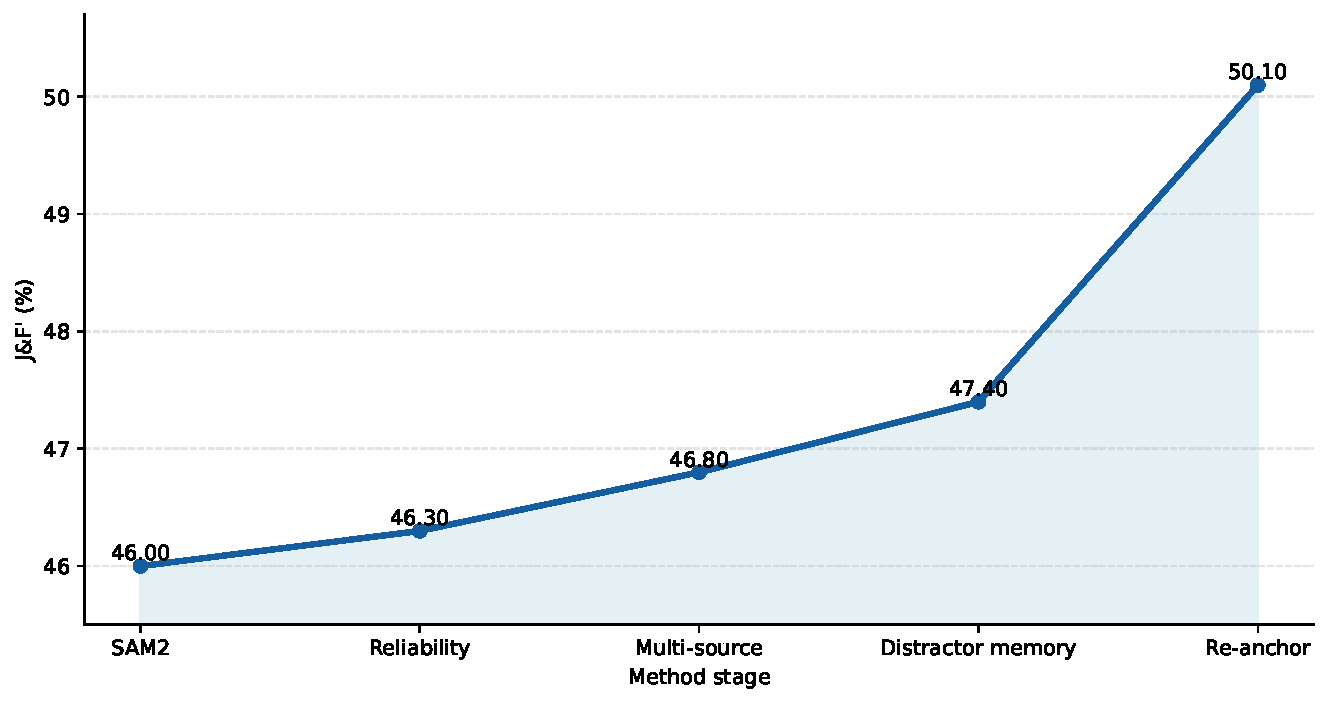
\includegraphics[width=0.78\linewidth]{figures/score_progression.pdf}
  \caption{完整测试上的阶段性 \jf{}。显著增益出现在候选再获取、身份验证与重锚定形成闭环之后。}
  \label{fig:score}
\end{figure}

\section{面向 15 个困难实例的 MLLM 上限研究}

完成整体结构优化后，我们没有继续在全量数据上堆叠提示，而是挑选 15 个仍具有明显身份歧义的序列作深入研究。目的并非用手工描述替代泛化模型，而是回答两个更具体的问题：其一，结构化提示能否激活 MLLM 对遮挡、物体交互和长程运动的理解；其二，这种“真正看懂视频内容”的能力在与候选生成和分割传播对齐后，最多能够修复到什么程度。因而，本节只使用单个视频对象的前后指标衡量针对性调整，不把这些结果混入前述全量成绩。

\begin{table}[H]
\centering
\caption{正文涉及的重点困难样本及内容简称。}
\label{tab:video-codes}
\small
\renewcommand{\arraystretch}{1.14}
\begin{tabularx}{\textwidth}{>{\raggedright\arraybackslash}p{2.25cm} >{\raggedright\arraybackslash}p{3.8cm} >{\raggedright\arraybackslash}X}
\toprule
样本编码 & 内容简称 & 核心困难 \\
\midrule
\code{z6dx46qr} & 低对比双黑点小目标 & 可辨识纹理极少，目标与背景对比度低 \\
\code{amfdu83t} & 边缘袋鼠重现 & 首帧仅露出局部，出画后在强同类干扰旁重现 \\
\code{q0sizv6m} & 多只小动物前景运动 & 目标靠近镜头、短暂消失，并从画面下缘重新出现 \\
\code{8jsm23a7} & 七条麻将拿取 & 手部遮挡和运动模糊造成身份转移，同类牌面高度相似 \\
\code{r13u5z4y} & 草莓切片移动 & 首帧严重遮挡，多块切片同时移动并相邻放置 \\
\code{4vznweiu} & 旋转字母骰子 & 目标极小、不断转面，邻近存在多枚同类骰子 \\
\code{1qlssuz2} & 车道内小车 & 远距离小目标沿固定车道运动并经历遮挡 \\
\bottomrule
\end{tabularx}
\end{table}

\subsection{为什么需要 MLLM，又为什么不能让它直接分割}
在麻将被拿起、袋鼠离场重现、小动物向镜头靠近等片段中，单帧外观相似度不足以解释物理过程。MLLM 的优势在于把离散观测组织为事件链，例如“拿起—手部遮挡—运动模糊—放到牌列左侧”或“朝镜头移动—从下边缘重现—后期离场”。但实践中，直接输入大尺寸多帧组合图会超时并稀释注意力；正确的语言故事也不等于正确候选框，更不等于像素边界。

为此本文结合 Qwen-VL 的图像理解能力\cite{bai2025qwen25vl}设计分层调用框架：第一层对每个关键帧的参考目标、全局上下文和候选叠加图做短视觉描述；超时帧自动缩为仅包含局部目标的重试。第二层由深度思考模型在纯文本上聚合可见状态、运动方向、遮挡关系和同类干扰物，输出支持、否决或不确定。MLLM 不直接产生最终掩码，也不得单独提升锚点；在同类密集场景中，不确定意味着拒绝写入，在极小目标场景中则保持基线。

\begin{table}[H]
\centering
\caption{针对性内容理解与重锚定的对象级结果。}
\label{tab:object-gains}
\small
\renewcommand{\arraystretch}{1.16}
\begin{tabularx}{\textwidth}{>{\raggedright\arraybackslash}p{3.8cm} >{\centering\arraybackslash}p{1.7cm} >{\centering\arraybackslash}p{1.7cm} >{\raggedright\arraybackslash}X}
\toprule
视频对象 & 调整前 \jf{} & 调整后 \jf{} & 主要有效证据 \\
\midrule
低对比小目标（\code{z6dx46qr:1}） & 40.47 & 65.14 & 更强视觉候选保持了低对比目标的连续性 \\
边缘袋鼠（\code{amfdu83t:1}） & 28.44 & 84.84 & 离场、左下重现和向镜头运动构成一致事件链 \\
前景小动物（\code{q0sizv6m:obj2}） & 12.34 & 68.29 & 向镜头靠近、下边缘重现与后续尺度变化相互印证 \\
\bottomrule
\end{tabularx}
\end{table}

\subsection{定性结果：真正有效的是“事件理解落到新锚点”}
\begin{figure}[H]
\centering
\begin{subfigure}[t]{0.47\textwidth}
  \centering
  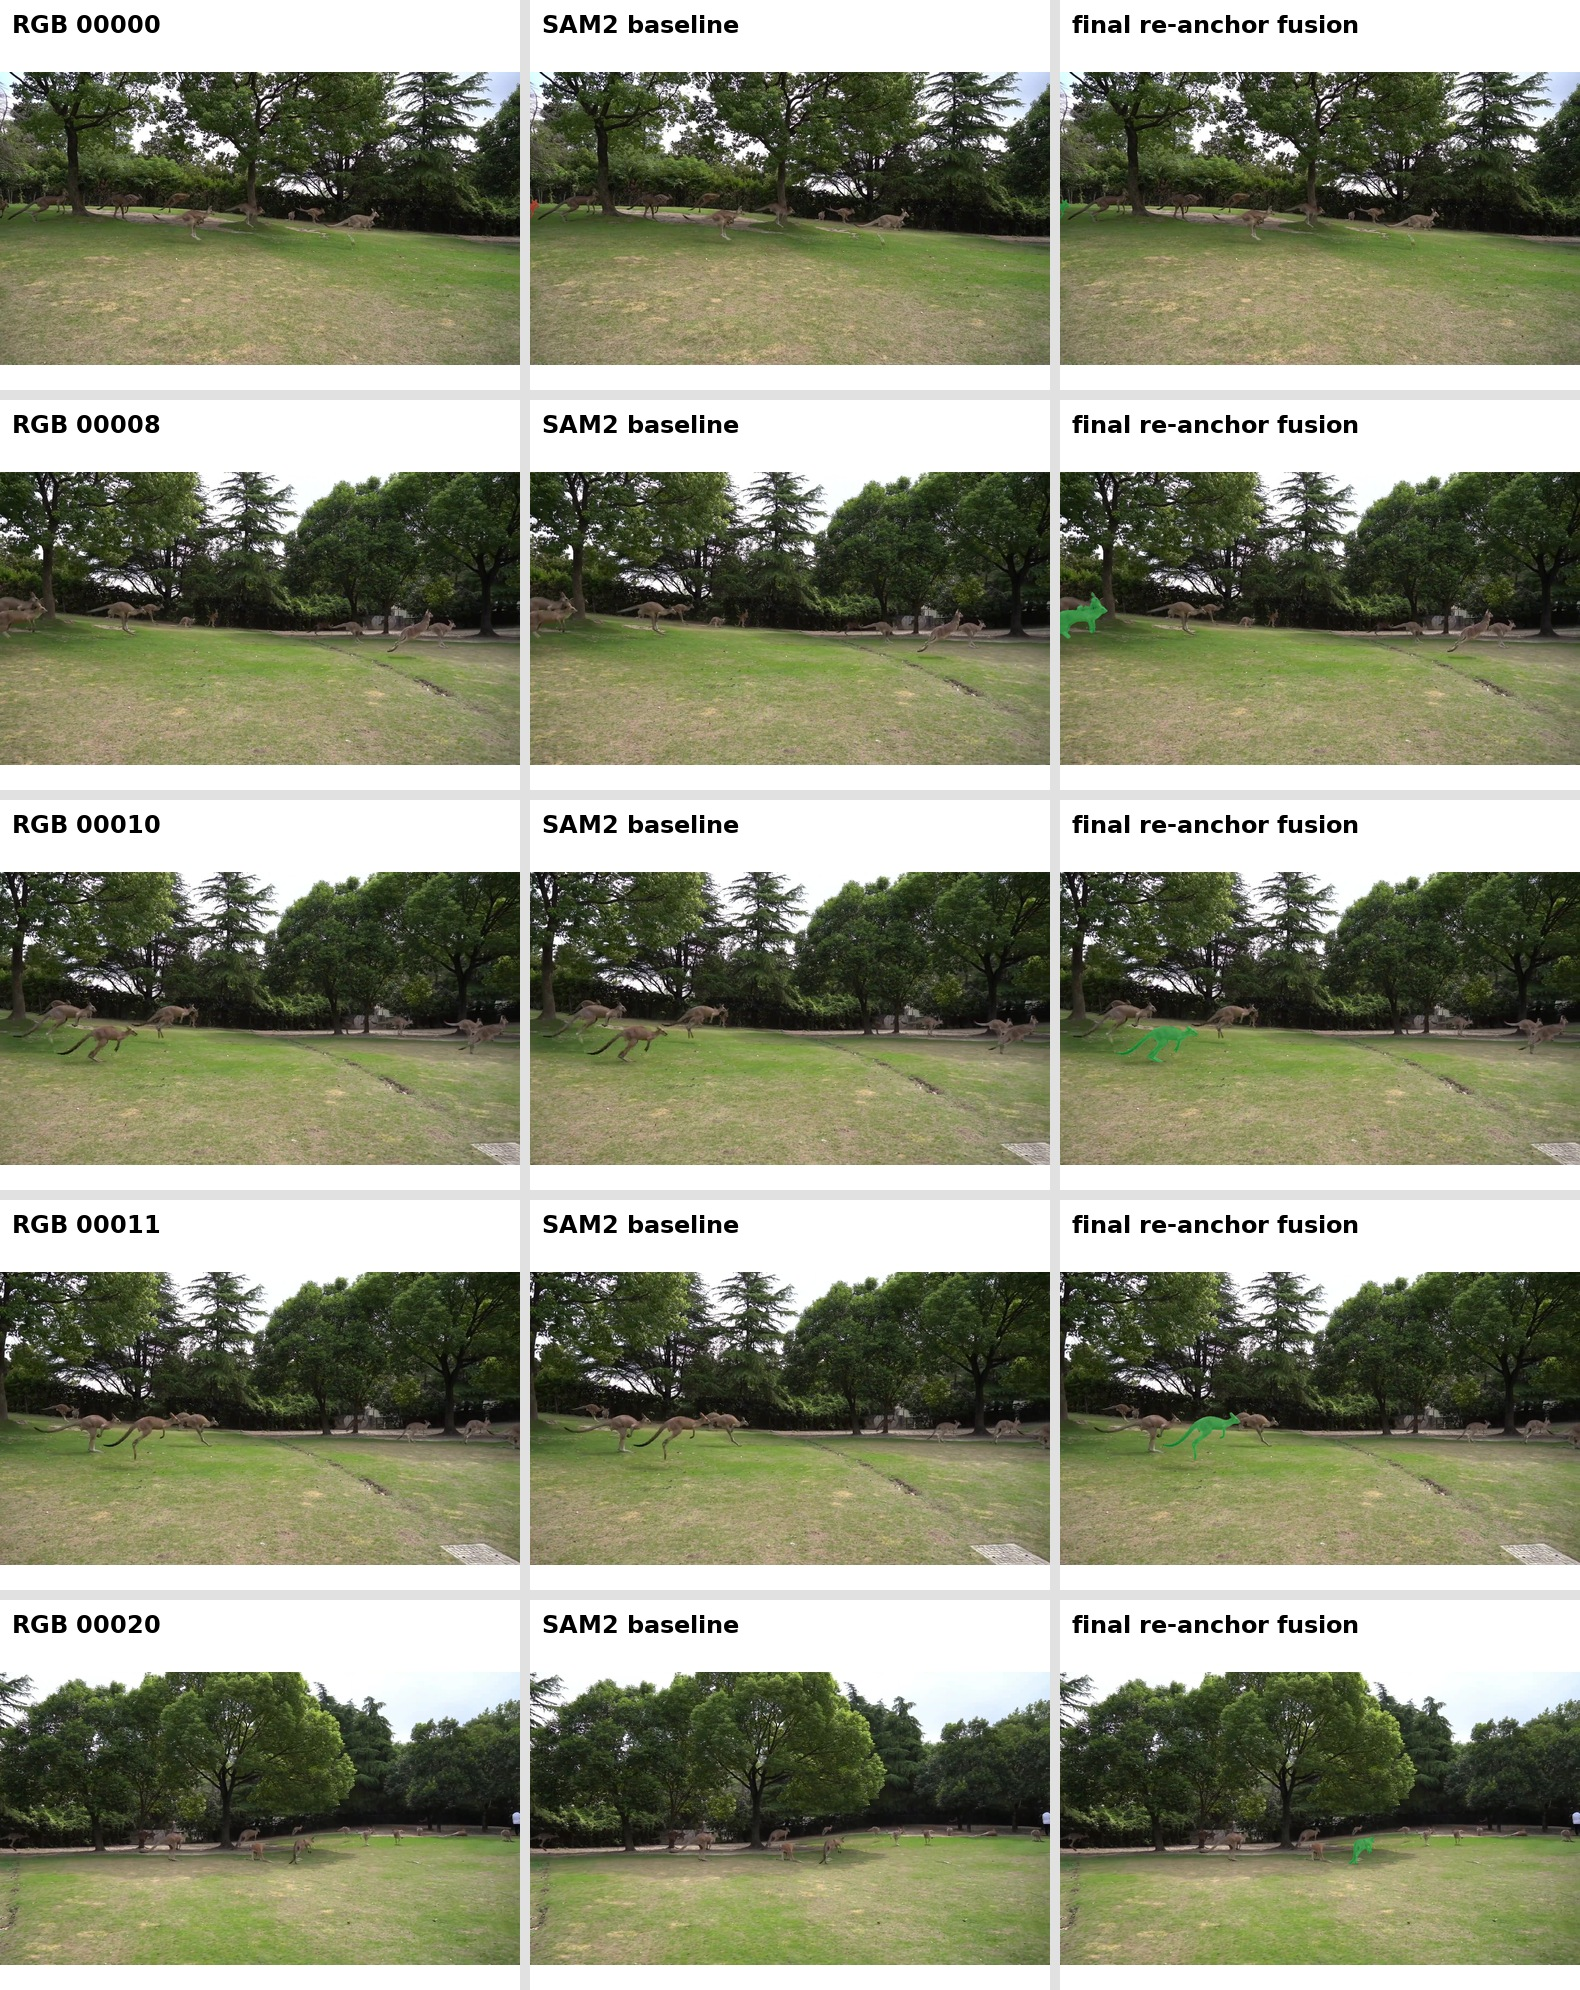
\includegraphics[width=\linewidth]{figures/amfdu_success.jpg}
  \caption{边缘袋鼠（\code{amfdu83t:obj1}）：首帧仅露出左边缘，目标离场后从左下靠近镜头重现。}
\end{subfigure}\hfill
\begin{subfigure}[t]{0.47\textwidth}
  \centering
  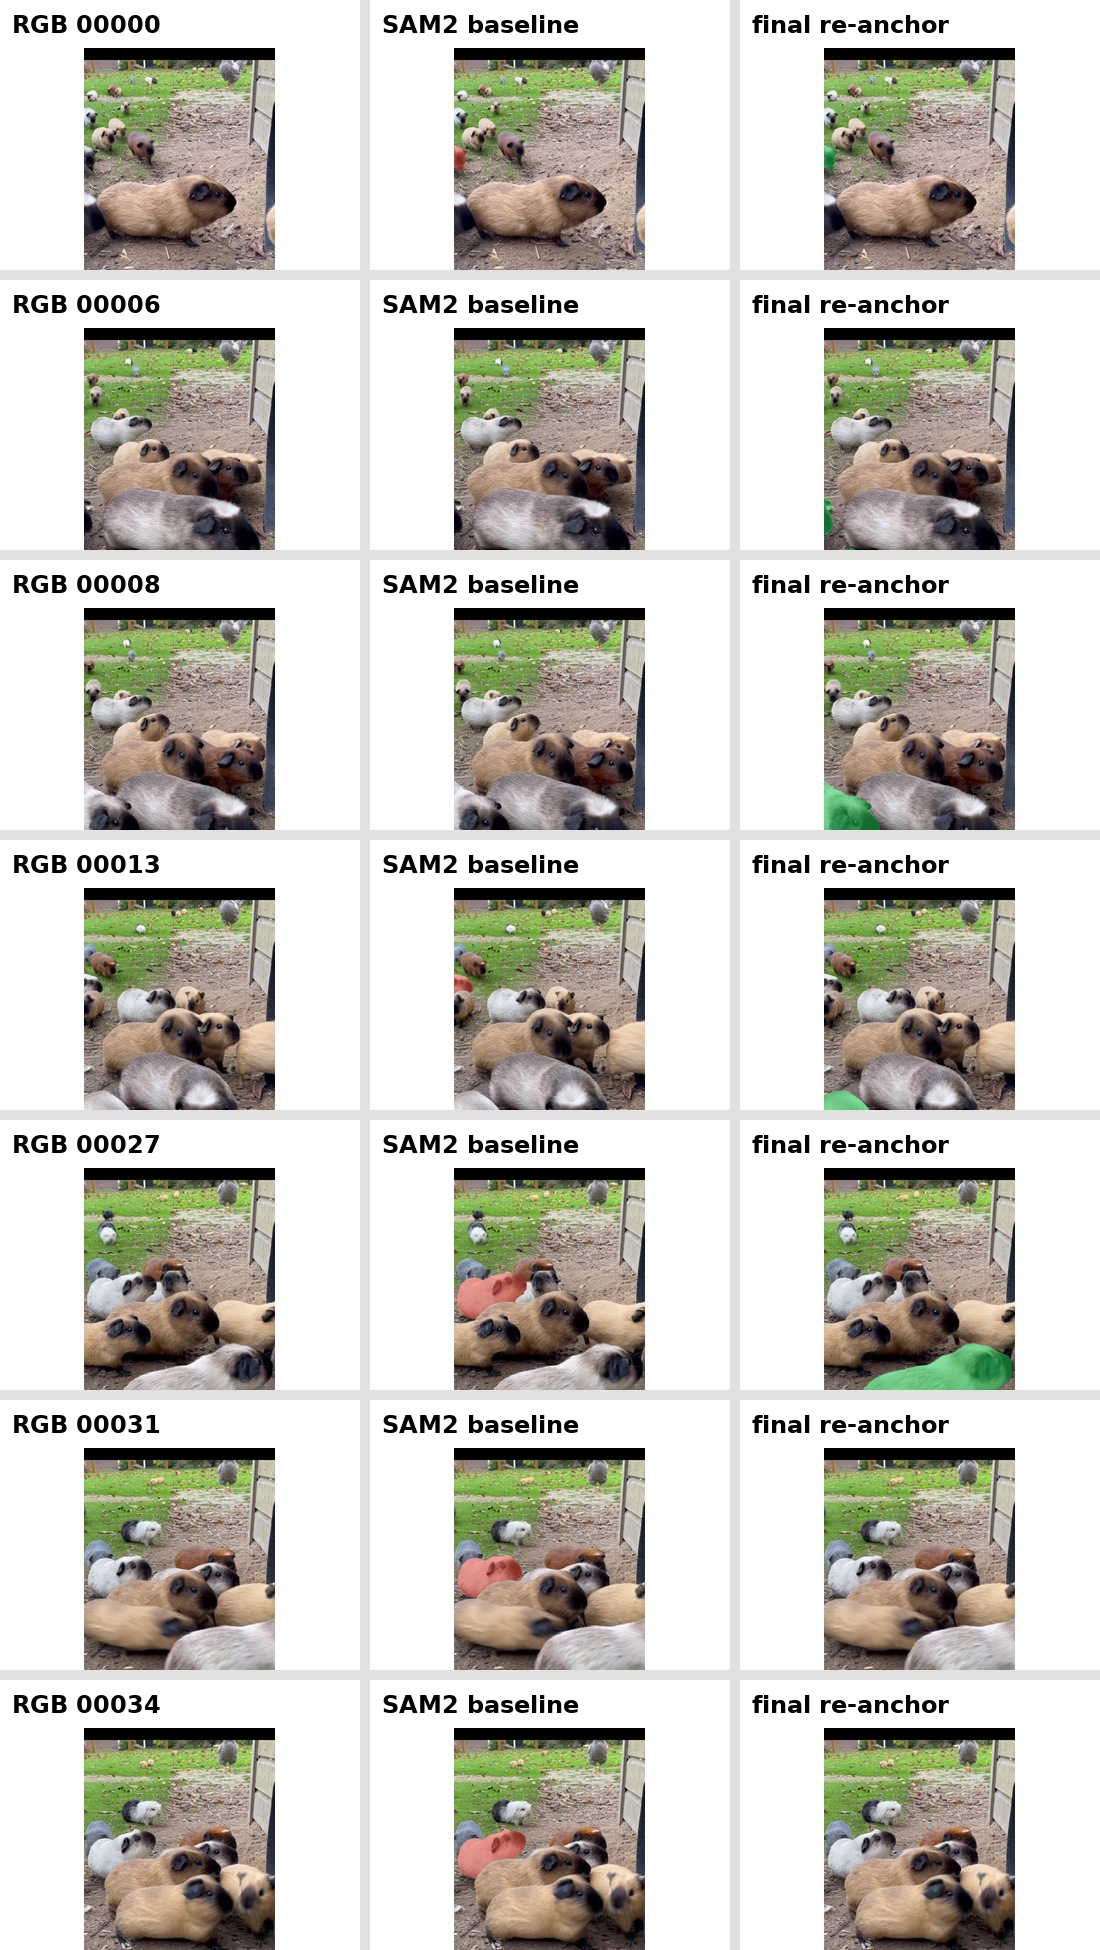
\includegraphics[width=\linewidth]{figures/q0_success_timeline.jpg}
  \caption{前景小动物（\code{q0sizv6m:obj2}）：目标向镜头运动并在下边缘重现，基线却锁定旧位置同类对象。}
\end{subfigure}
\caption{两个被平台明细验证的重锚定案例。绿色为最终融合，红色为基线。MLLM 的价值不在“看懂类别”，而在为后续候选生成提供可检验的时空约束。}
\label{fig:success}
\end{figure}

边缘袋鼠样本（\code{amfdu83t:obj1}）的首帧目标只占全图约 $0.052\%$，且仅露出头颈与前足；镜头移动后目标出画，左侧长期存在另一只更完整、更显眼的袋鼠。事件账本把第 8 帧附近左下方快速靠近镜头的袋鼠视为“原对象重现”候选，经锚点注入后，对象分升至 84.84。这里真正起作用的是候选位置、后续运动和 SAM2 回传形成闭环，而不是一句“这是袋鼠”。

多只小动物前景运动样本（\code{q0sizv6m:obj2}）中，各实例外观高度相似。目标先向镜头靠近并短暂消失，第 6--8 帧从画面下方逐渐出现；原始模型却在后期锁定旧位置附近的另一只同类对象。MLLM 将“向前景运动—下边缘重现”转化为搜索约束，候选框提示再驱动 SAM2 有界传播，使对象分由 12.34 升至 68.29。不过第 31 帧附近仅剩臀部边缘、第 34 帧后应消失，当前输出仍有晚期误检，说明账本还需更严格地区分可见、局部可见和缺席状态。

\subsection{失败案例揭示的边界}
\begin{figure}[H]
  \centering
  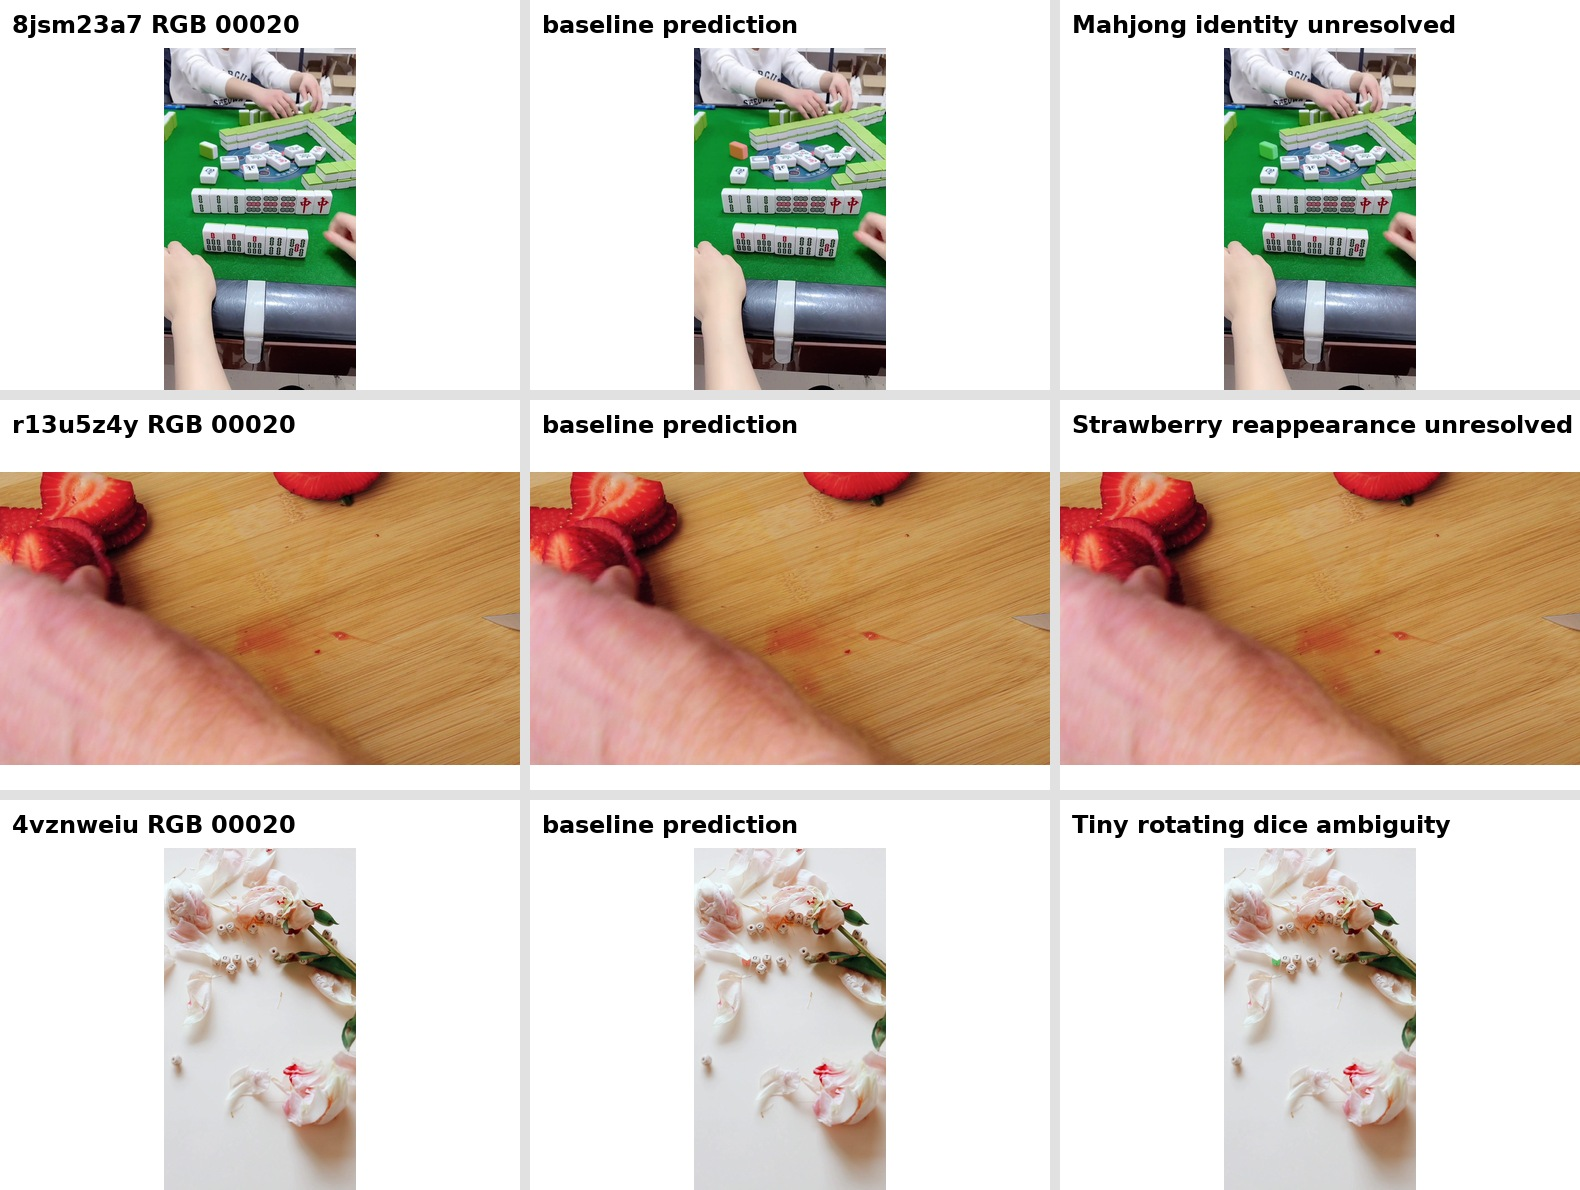
\includegraphics[width=0.88\linewidth]{figures/remaining_failures.jpg}
  \caption{仍未解决的代表性困难：麻将身份转移、草莓切片同类重现与旋转字母骰子。单帧“合理非空”并不等价于同一实例。}
  \label{fig:failures}
\end{figure}

\textbf{七条麻将拿取（\code{8jsm23a7}）}：首帧目标背面朝上，第 1 帧被手遮挡，第 3--5 帧在拖影中短暂显露七条特征，第 6--7 帧被放到面前牌列最左侧。早期提示把“左侧牌”语言化得过强，实际候选落在远处牌列的二条，说明用户叙述和 MLLM 推理必须绑定候选编号与像素证据，不能直接变成坐标暗示。

\textbf{草莓切片移动（\code{r13u5z4y}）}：首帧只露出被遮挡的一小段边缘，之后与另一切片同时被手移动，重现时周围已有多个近似切片。当前系统能安全拒绝错误草莓，却无法稳定枚举并分离正确切片；这是候选生成失败，而不是验证阈值问题。

\textbf{旋转字母骰子（\code{4vznweiu}）}：目标极小且不断转面，表面字母随视角改变，邻近还有多枚相似骰子。高分辨率局部裁剪只解决“看不清”，不解决“认不出”。需要先为所有同类骰子建立独立轨迹和多面外观记忆，再根据相对运动选择实例。

\section{讨论：当前缺陷与前沿改进方向}

\subsection{为什么训练自由系统仍会遇到上限}
当前系统已经具备完整控制闭环，但正确实例未进入候选池时，任何描述器和 MLLM 都只能安全拒绝；若多个同类对象在可见信息上完全不可辨识，单帧模型也无法凭空恢复身份。另一个限制是手工事件账本的状态边界不够精细：它能描述“重现”，却未必准确决定每一帧的 partial/absent；过长的重传播窗口会把局部正确锚点扩散成后期误检。

对象级结果说明，MLLM 确实能在少数具有清晰物理事件链的样本上显著扩大恢复上限，但这种能力尚未覆盖全部难例。麻将、草莓切片和旋转骰子仍然缺少足够可靠的候选分离；仅修改提示词无法弥补像素候选缺失。剩余高潜力对象的共同要求是“全视频候选枚举 + 每个同类实例独立记忆 + 显式缺席状态 + 双向一致性”，而不是继续进行几乎不改变轨迹的阈值实验。

\subsection{结合前沿的后续路线}
\textbf{（1）对象图与逐对象记忆治理。} SAM2Long 已证明训练自由的记忆树能够缓解贪心路径造成的错误累积\cite{ding2024sam2long}；DAM4SAM 说明相似干扰物应被显式写入负例记忆，而不是只在输出端过滤\cite{videnovic2024dam4sam}。OAMVOS 又把可靠性状态、分支恢复和延迟记忆晋升组合起来\cite{oamvos2026}。对多目标场景，SAM3-DMS 指出按整组对象的平均置信度统一更新会掩盖某个消失目标的失败，因此把 memory selection 解耦为逐对象决策\cite{shen2026sam3dms}。这些工作共同支持本文的下一步：将每个同类候选建成独立节点，以光流、可达速度、遮挡关系和正负特征差连边，在可见、局部可见和缺席三种状态间搜索全局最合理的身份路径；只有得到未来帧持续支持的分支才晋升长期记忆。

\textbf{（2）让 SAM3 提供候选，让对象证据决定身份。} SAM~3 从 SAM2 的可提示视觉分割进一步扩展到可提示概念分割：短名词短语、图像样例或二者组合均可驱动检测、分割和跟踪；其 detector--tracker 结构与 presence head 将识别和定位适度解耦\cite{carion2025sam3}。这种能力适合枚举后续帧中的同类候选，却仍不能回答“它是不是首帧那一只”。TEP 按常规、小目标和语义主导目标分路由，并用外部 tracker 与 MLLM 增强提示\cite{zhang2026tep}；Re-Prompting SAM~3 则先检测后续候选，再用 DINOv3 对象检索选择新锚点\cite{gao2026reprompt}。AgentRVOS 进一步主张先生成对象轨迹证据，再让 MLLM 逐轮筛选，而不是让语言模型在缺少对象级证据时先决定关键帧\cite{agentrvos2026}。因此更合理的组合是：SAM3 负责高召回候选，视觉描述器和对象图负责实例选择，SAM2 或 SAM3 tracker 只传播经过确认的锚点。

\textbf{（3）把跨镜头变化与连续运动分开处理。} 当前 15 个难例主要由遮挡和同类干扰造成，但真实互联网视频还包含镜头剪辑和视角跳变。SAAS 通过转场模拟增强、转场检测和转场理解处理多镜头 VOS，并建立 Cut-VOS benchmark\cite{hu2026saas}。这提示后续状态机应先判断“对象运动”还是“镜头切换”：前者依赖物理可达性，后者不能沿用原运动模型，而应重新依靠语义和对象检索建立锚点。

\textbf{（4）在训练层学习“何时记、记什么、何时缺席”。} 训练自由策略依赖人工阈值和有限特征，难以校准不同目标的身份不确定性。可训练方向不是简单微调 mask decoder，而是加入三类监督：目标与干扰物的对比式记忆损失；遮挡前后同一实例的一致性与跨实例间隔；对可见、局部可见、缺席和锚点晋升的序列决策监督。Cutie 的对象级记忆读取\cite{cheng2024cutie}和 AOT 的多对象关联\cite{yang2021aot}可作为结构基础；训练时还可用遮挡合成、同类替换和视角变换构造困难负例。这样，MLLM 产生的事件标签可以成为弱监督，而不必在运行时承担唯一判断责任。

\subsection{课程学习体会}
{\small
\begin{enumerate}[label=\arabic*.,leftmargin=2.2em,itemsep=0.3em]
  \item 赵老师讲课深入浅出，清晰易懂，渴望让教学内容结合实践/落地前沿的出发点也很好，您提出的以后要讲学结合、翻转课堂的想法我觉得之后学期值得一试，让同学们深入实践、自己尝试做明白、讲清楚，很可能掌握更多。
  \item 针对您的教学内容，我并无不满，仅有以下拙见供您参考：私以为结合Transformer、CNN等基础网络结构的知识（这一方面是承前启后的必要知识点，另一方面也是以我个人为例，不需要担心之前是否学过，因为每次再学都会认识到淡忘的要点和新的深入体会，确为常学常新），讲一些当前计算机视觉领域前沿具体的课题任务（譬如目标检测、分割、跟踪和视觉理解、生成的多模态大模型相关等等）和前沿也绕不开的“高级基础模型”（比如DiT、YOLO、SAM等等）为什么厉害、强在哪里、设计理念等，这是我个人比较渴望学到，而且也难找到其他媒体资源系统地、由浅入深地来讲“好”的知识。
  \item 您邀请您的研究生学生和业界合作者来分享都是很好的想法，既带来前沿的研究介绍，也为我们提供和前沿研究者沟通交流的机会，只是同学们部分有些内敛，您不必介意，万望坚持。不过一个明显的点，不管是从个人了解来说还是分享所见来看，cv的调研要么是交叉结合的落地工程实践要么是转向多模态这一块，传统cv的工作绝大部分都变成了基础知识了；另一方面要调整教学内容也可能需要对PPT大动干戈、花心思备课，同学们可能也不尽乐意听，费力不讨好，所以我以上的拙见都不见得有建设性，万望您包容见谅，这也都是教学和实际稍有矛盾需要细细考量的点吧。最后，感谢赵老师一学期尽心竭力地教学付出，于我的确受益良多，祝赵老师工作顺利、身体健康；也感谢助教负责与耐心，祝助教学长们paper都ac。
\end{enumerate}
}

\section{结论}
本文以 SAM2 在 MOSEv2 上的复现和改进为主线，针对复杂遮挡、重现、同类干扰和极小目标，提出训练自由的对象中心重锚定系统。系统保留 SAM2 在连续可见区间的优势，同时增加三态审计、正负身份记忆、高召回候选、延迟提交、有界回传和保守融合。面向一般场景的完整测试取得 50.1 的 \jf{}，较复现基线提高约 4 个点。完成整体改进后，本文再以 15 个困难实例研究 MLLM 提示和长程视频理解的作用上限；其中边缘袋鼠和前景小动物两个对象分别由 28.44、12.34 提升至 84.84、68.29，证明高层事件理解只有落实为可验证候选和局部重传播时才会转化为像素收益。

实验的价值不仅是最高分，而是明确了有效改动的层级：输出门控可以少犯错，只有经验证的后续锚点才能真正恢复目标；MLLM 可以解释物理过程，却必须与候选 ID、对象特征和时序几何对齐，才能产生正确像素。未来应把手工账本升级为显式多对象图和可学习的干扰感知记忆，并利用 SAM3 的语义候选能力补足召回，而不是再次退回单路径、单阈值的传播范式。

\bibliographystyle{unsrt}
\bibliography{reference}

\end{document}
